\documentclass{article}

% Formatting
\DeclareUnicodeCharacter{2060}{\nolinebreak} % Prevent unicode (U+2060) error on local complile
\frenchspacing % No double spacing between sentences
\hbadness=1000000 % Turn off \hbox badness warnings
\linespread{1.2} % Set linespace


% Packages
\usepackage[a4paper, left=1.5cm, right=1.5cm, top=1.5cm, bottom=1.5cm]{geometry}
\usepackage{array} % For allowing new column types in tables
\usepackage{authblk} % For author formatting
\usepackage{caption} % For figure and table captions
\usepackage{cclicenses} % For creative commons license
\usepackage{float} % To force figure location after text
\usepackage{graphicx} % Adds more functionality to graphics for inclusion of figures
\usepackage{lscape} % For landscape pages
\usepackage{lineno} % Allows use of \linenumbers to add line numbers 
\usepackage{lmodern} % A scalable font - avoids erros due to non-sclabale fonts
\usepackage{longtable,booktabs}  % For tables
\usepackage{markdown} % allow use of markdown syntax
\usepackage{microtype} % 'Improved' typesetting
\usepackage[nottoc,numbib]{tocbibind} % Add references to table of contents
\usepackage{parskip} % Adds white space between paragraphs
\usepackage{pdflscape} % To create landscape pages that show as landscape in PDF viewer
\usepackage{ragged2e} % Better right ragged edges (allows hyphenation)
\usepackage{subcaption} % Allows use of subfigures and subtables
\usepackage{subfig} % Allows use of subfigures and subtables
\usepackage[super]{natbib} % Citations using superscript
\usepackage{titlesec} % For title spacing
\usepackage[toc,page]{appendix}
\usepackage{url} % Tidy web links
\usepackage[utf8]{inputenc}
\usepackage{verbatim}
\usepackage{xcolor} % For coloured text
\usepackage{xurl} % For url but with more flexible linebreaking


% Choose your own colour
\usepackage{color}
\newcommand{\mjanote}[2][\textcolor{red}{\dagger}]{\textcolor{red}{$#1$}\marginpar{\color{red}\raggedright\tiny$#1$ #2}}
\newcommand{\mjaFIXME}[1]{\textcolor{red}{[\textbf{FIXME} \textsl{#1}]}}
\newcommand{\kpnote}[2][\textcolor{magenta}{\dagger}]{\textcolor{magenta}{$#1$}\marginpar{\color{magenta}\raggedright\tiny$#1$ #2}}
\newcommand{\kpFIXME}[1]{\textcolor{magenta}{[\textbf{FIXME} \textsl{#1}]}}


% Info on wordcounts:
% https://www.overleaf.com/learn/how-to/Is_there_a_way_to_run_a_word_count_that_doesn%27t_include_LaTeX_commands%3F

% To include refs in word count:
%TC:incbib


\newcommand{\detailtexcount}[1]{%
  \immediate\write18{texcount -merge -sum -q #1.tex output.bbl > #1.wcdetail }%
  \verbatiminput{#1.wcdetail}%
}

\newcommand{\quickwordcount}[1]{%
  \immediate\write18{texcount -1 -sum -merge -q #1.tex output.bbl > #1-words.sum }%
  \input{#1-words.sum} words%
}

\newcommand{\quickcharcount}[1]{%
  \immediate\write18{texcount -1 -sum -merge -char -q #1.tex output.bbl > #1-chars.sum }%
  \input{#1-chars.sum} characters (not including spaces)%
}

% Count tables in wordcount

%TC:group table 0 1
%TC:group tabular 1 1

\begin{document}


% Ignore title and abstract in word count
%TC:ignore
\title{Title}


\renewcommand{\thefootnote}{\fnsymbol{footnote}}
\author[1,2]{Kerry Pearn}
\author[*1,2]{Michael Allen}
\author[1,2]{Martin James}

% Check affiliations - update RDE Name
\affil[1]{\footnotesize University of Exeter Medical School}
\affil[2]{\footnotesize NIHR South West Peninsula Applied Research Collaboration (ARC).}
\affil[*]{\footnotesize Corresponding author: m.allen@exeter.ac.uk}
%TC:endignore

\section{Introduction}

% Include
% 1) What is the problem?
% 2) What do we know about low and varying use of thrombolysis
% 3) What do we not know
% 4) How are we addressing what we don't know

% 1) What is the problem?

Stroke remains one of the top three global causes of death and disability \cite{feigin_global_2021}. Despite reductions in age-standardised rates of stroke, ageing populations are driving an increase in the absolute number of strokes \cite{feigin_global_2021}. Across Europe, in 2017, stroke was found to cost healthcare systems \texteuro 27 billion, or 1.7\% of health expenditure \cite{luengo-fernandez_economic_2020}. Thrombolysis with recombinant tissue plasminogen activator, can significantly reduce disability after ischaemic stroke, so long as it is given in the first few hours after stroke onset \cite{emberson_effect_2014}. Despite thrombolysis being of proven benefit in ischaemic stroke, use of thrombolysis varies significantly both between and within European countries \cite{aguiar_de_sousa_access_2019}. In England and Wales the national stroke audit reported that in 2021/22, 20 years on from the original European Medicines Agency licencing of alteplase for acute ischaemic stroke, thrombolysis rates for emergency stroke admissions varied from just 1\% to 28\% between hospitals \cite{sentinel_national_stroke_audit_programme_ssnap_2022}, with a median rate of 10.4\% and an inter-quartile range of 8\%-13\%, against a 2019 NHS England long term plan that 20\% of patients of emergency stroke admissions should be receiving thrombolysis \cite{nhs_long_term_plan_2019}.

The NHS plan for improving stroke care also sets a target that patients should receive thrombolysis within 60 minutes of arrival, but ideally within 20 minutes (12). Whilst this speed of thrombolysis, called door-to-needle time, provides an ambitious target, it has been shown to be achievable as Helsinki University Central Hospital has reported a median door-to-needle time of 20 minutes, with 94\% of patients treated within 60 minutes \cite{meretoja_reducing_2012}.

% 2) What do we know about low and varying use of thrombolysis

Studies have shown that reasons for low and varying thrombolysis rates are multi-factorial. Reasons include late presentation \cite{aguiar_de_sousa_access_2019}, lack of expertise \cite{aguiar_de_sousa_access_2019} or lack of clear protocols or training \cite{carter-jones_stroke_2011}, delayed access to specialists \cite{kamal_delays_2017}, and poor triage by ambulance or emergency department staff \cite{carter-jones_stroke_2011}. For many factors, the establishment of primary stroke centres has been suggested to improve the emergency care of patients with stroke and reduce barriers to thrombolysis \cite{carter-jones_stroke_2011}, with a centralised model of primary stroke centres leading to increased likelihood of thrombolysis \cite{lahr_proportion_2012, morris_impact_2014, hunter_impact_2013}. 

In addition to organisational factors, clinicians can have varying attitudes to which patients are suitable candidates for thrombolysis. In a discrete choice experiment \cite{de_brun_factors_2018}, 138 clinicians considered hypothetical patient vignettes, and responded as to whether they would give the patients thrombolysis. The authors concluded that there was considerable heterogeneity among respondents in their thrombolysis decision-making. Areas of difference were around whether to give thrombolysis to mild strokes, to older patients beyond 3 hours from stroke onset, and when there was pre-existing disability.

Based on national audit data from three years of emergency stroke admissions, we have previously built models of the emergency stroke pathway using clinical pathway simulation to examine the potential scale of the effect of changing two aspects of the stroke pathway performance (1. the in-hospital process speeds, and 2. the proportion of patients with a determined stroke onset time), and using machine learning to examine the effect of replicating clinical decision-making around thrombolysis from higher thrombolysing hospitals to lower thrombolysing hospitals \cite{allen_using_2022, allen_use_2022}. The machine learning model learned whether any particular patient would receive thrombolysis in any particular emergency stroke centre. Using these models we found that it would be credible to target an increase in average thrombolysis in England and Wales, from 11\% to 18\%, but that each hospital should have its own target, reflecting differences in local populations. We found that the largest increase in thrombolysis use would come from replicating thrombolysis decision-making practice from higher to lower thrombolysing hospitals. Two other important factors influencing thrombolysis rates were determination of stroke onset time in some hospitals, and improving the speed of the in-hospital thrombolysis pathway.

% 3) What do we not know

In our previous work we established that we could predict the use of thrombolysis in patients arriving within 4 hours of known stroke onset with 84.3\% accuracy \cite{allen_use_2022}. We could then ask the question "What if this patient attended another hospital - would they likely be given thrombolysis?" In that work, when we altered selection of patients for thrombolysis, we were only predicting thrombolysis choice; we were not examining outcomes after stroke with and without thrombolysis, which left open the question of whether stroke teams with higher thrombolysis use were likely to be achieving better outcomes. In this paper we extend the pathway model to examine outcomes after applying the predicted decision-making from higher thrombolysing hospitals, including a health economics analysis.
\section{Methods}

\subsection{Data}

Data was used for all emergency stroke admissions to England and Wales for the 5 years 2017-2021, for teams with average admissions of at least 100 per year. The total number of patients were, 301,747, of which 114,277 (38\%) arrived within 4 hours of known stroke onset. Of those arriving within 4 hours of known stroke onset 102,971 (90\%) arrived by ambulance. Outcome modelling is based on all arrivals, but the stroke pathway modelling is based on those arriving by ambulance within 4 hours of known stroke onset.



\subsection{Overview}

\begin{figure}
    \centering
    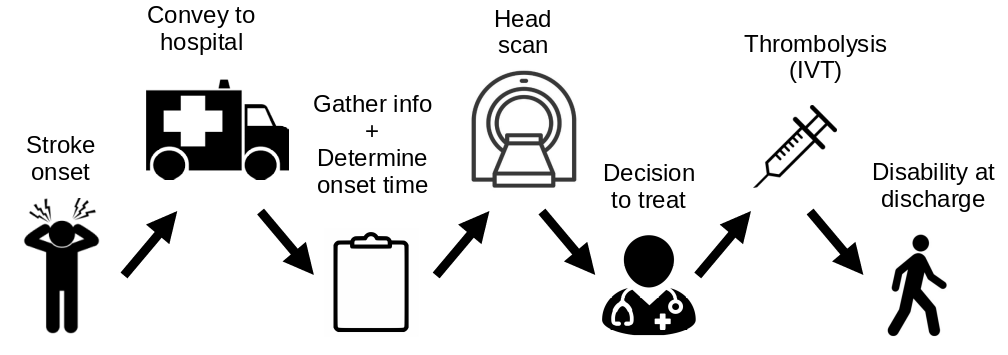
\includegraphics[width=0.75\linewidth]{images/flow}
    \caption{Enter Caption}
    \label{flow}
\end{figure}

\subsection{Thrombolysis decision model}

\subsection{Stroke outcome machine learning model}

\subsection{Lifetime economic model}

\subsection{Pathway model}

\subsection{Code and artificial patients}
\section{Results}

Descriptive statistics for hospital processes and patient populations are shown in the supplementary material.

\subsection{Thrombolysis decision model}

The thrombolysis decision model predicted the probability of any patient receiving thrombolysis at any given stroke team.

Using an 80:20 train:test split, the model had an accuracy of 85\%, a balanced accuracy of 82\% (accuracy and balanced accuracy using a 50\% probability cut-off to classify a patient as a binary `likely to receive thrombolysis' or not), and a receiver operating characteristic area under curve of 0.92.


\subsection{Stroke outcome machine learning model}

Using a 4:1 train:test split, the model had a receiver operating characteristic area under curve of 0.80.

\subsection{Benchmark stroke teams and benchmark decisions}

\textit{Benchmark decisions} are those that would likely be taken by the majority 25 \textit{benchmark} stroke teams most likely to use thrombolysis (if all stroke teams saw the same patients). If all decisions-to-treat were made according to benchmark decisions, average thrombolysis across stroke teams would increase from 36\% to 45\% (in the modelled patient population). Thrombolysis use in the 25 stroke teams least likely to use thrombolysis would increase from 29\% to 46\%.

\subsection{Prototype patients}

\subsubsection{Thrombolysis decisions in prototype patients}

Prototype patients revealed variation in likely decisions between stroke teams (figure \ref{fig:thrombolysis_rates_prototype_patients}). While almost all stroke teams would give thrombolysis to the \textit{ideal} candidate for thrombolysis, the predicted use of thrombolysis varied more as one characteristic was changed from the \textit{ideal} candidate. In particular there was a very wide range in likelihood of a patient with a mild stroke (NIHSS 3) receiving thrombolysis. Mild stroke (NIHSS 0-4) represents a large proportion of admissions (54\% of all emergency stroke admissions, and 38\% of ischaemic stroke patients arriving by ambulance within 4 hours of known stroke onset). Combinations of \textit{non-ideal} patient characteristics reduced predicted use of thrombolysis further (again with significant variation between stroke teams), especially when the non-ideal characteristic was a mild stroke.

\begin{figure}
    \centering
    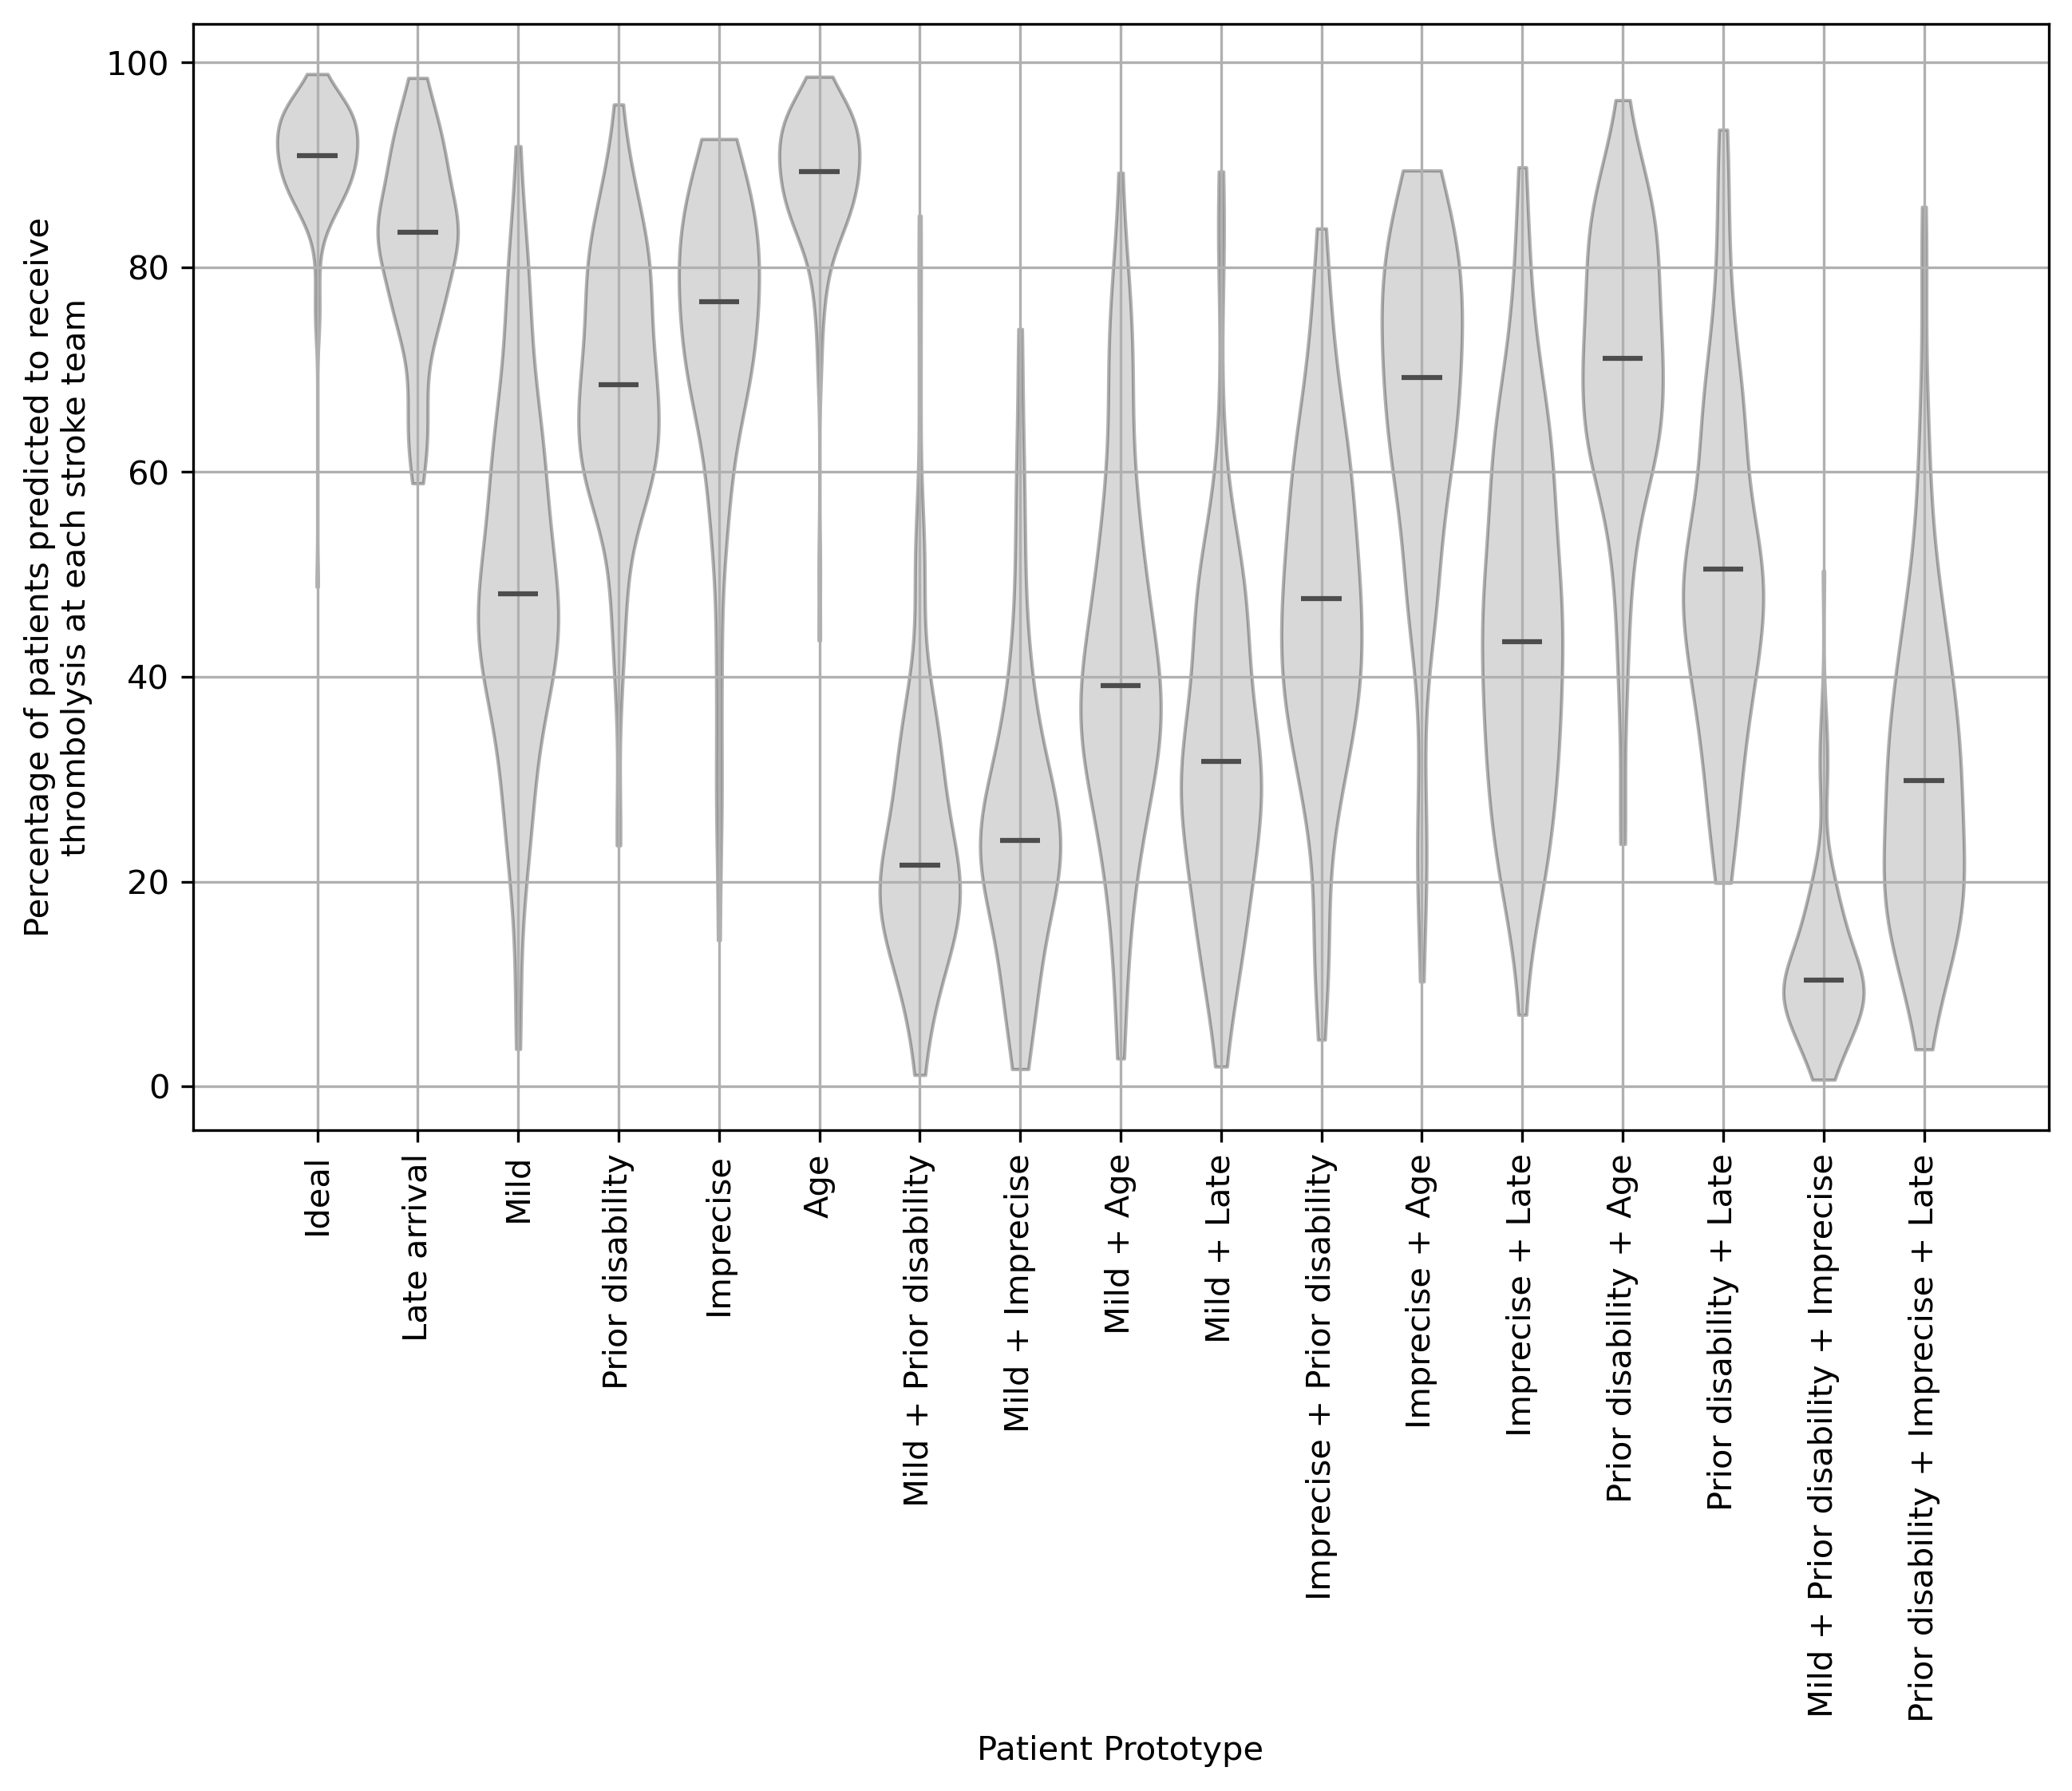
\includegraphics[width=0.75\linewidth]{images/prototype_patients_all_teams}
    \caption{Violin plots showing the variation in predicted thrombolysis rates for 17 patient prototypes across stroke teams. \textit{Ideal}: onset-to-arrival = 90 minutes; arrival-to-scan = 15 minutes; onset-to-thrombolysis = 120 minutes; stroke severity (NIHSS) = 15; pre-stroke disability (mRS) = 0; age = 72.5; precisely known onset; onset not during sleep; stroke type = infarction; patient has no atrial fibrillation and is not receiving anticoagulants for atrial fibrillation; \textit{Late arrival}: as \textit{ideal} but onset-to-arrival = 225 minutes and onset-to-thrombolysis = 255 minutes; \textit{Mild}: As \textit{ideal} but stroke severity = 3; \textit{Prior disability}: as \textit{ideal} but pre-stroke disability = 3; \textit{Imprecise}: as \textit{ideal} but stroke onset time estimated; \textit{Age}: as \textit{ideal} but age = 87.5.}
    \label{fig:thrombolysis_rates_prototype_patients}
\end{figure}

Figure \ref{fig:thrombolysis_rates_prototype_patients_team_x} shows an example of thrombolysis decisions for prototype patients in one stroke team, which is especially unlikely to give thrombolysis to patients with mild stroke, comparing likely use of thrombolysis to \textit{benchmark} hospitals.

\begin{figure}
    \centering
    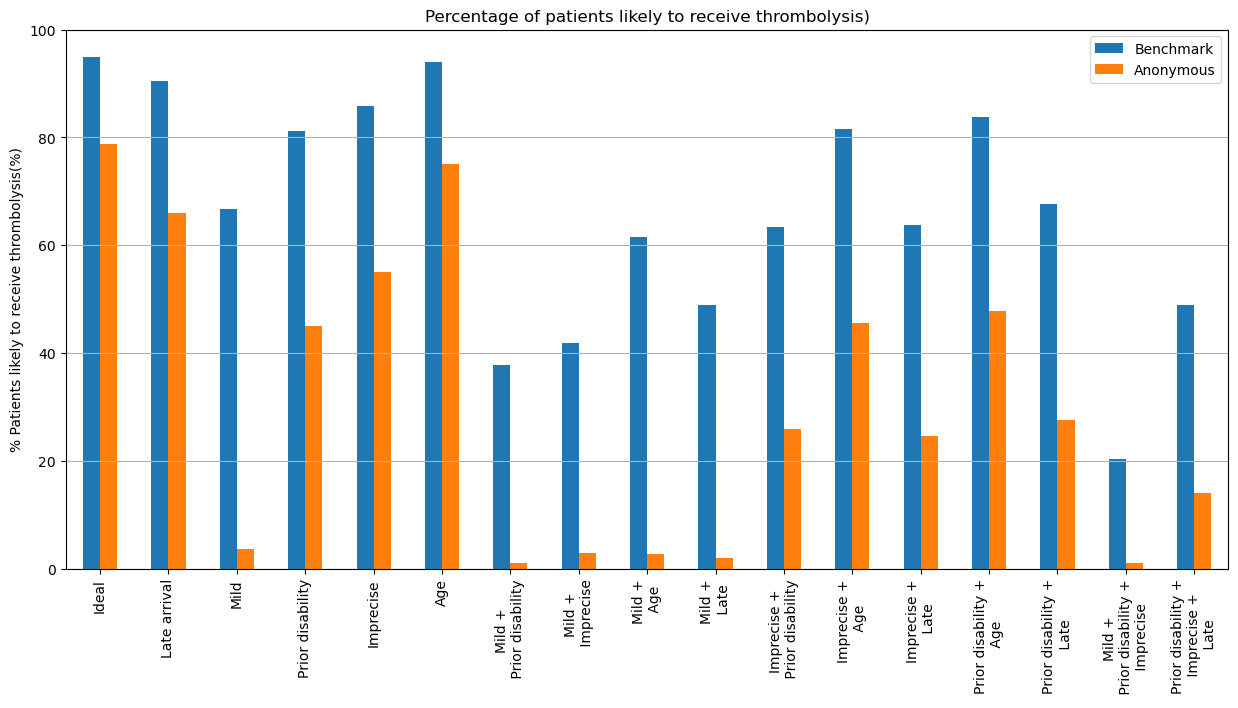
\includegraphics[width=1\linewidth]{images/prototype_patients_team_x.png}
    \caption{Predicted use of thrombolysis in 17 patient prototypes at a single hospital. Results show the the percentage of patients likely to receive thrombolysis, comparing \textit{benchmark decisions} (blue) and decisions likely at the example hospital (orange). Patient prototypes were: \textit{Ideal} candidate characteristics: onset-to-arrival = 90 minutes; arrival-to-scan = 15 minutes; onset-to-thrombolysis = 120 minutes; stroke severity (NIHSS) = 15; pre-stroke disability (mRS) = 0; age = 72.5; precisely known onset; onset not during sleep; stroke type = infarction; patient has no atrial fibrillation and is not receiving anticoagulants for atrial fibrillation. \textit{Late arrival}: as \textit{Ideal} but onset-to-arrival = 225 minutes and onset-to-thrombolysis = 255 minutes; \textit{Mild}: As \textit{Ideal} but stroke severity = 3; \textit{Prior disability}: as \textit{Ideal} but pre-stroke disability = 3; \textit{Imprecise}: as \textit{Ideal} but stroke onset time estimated. \textit{Age}: as \textit{Ideal} but age = 87.5. With combinations of non-ideal features.}
    \label{fig:thrombolysis_rates_prototype_patients_team_x}
\end{figure}


\subsubsection{Expected outcomes in prototype patients}

Figure \ref{fig:example_patient_outcomes} shows examples of outcome prediction for an \textit{ideal} candidate for thrombolysis, and a patient who is otherwise the same but has mild stroke. Expected benefit from thrombolysis may be calculated as the change in the proportion of \textit{good outcomes} (e.g. mRS 0-2), the proportion of \textit{bad outcomes} (e.g. mRS 5-6), or the shift in the central point of the outcome distribution (by weighting each mRS level by the probability of being discharged with that level of disability). 


\begin{figure}[h]
    \centering
    \begin{subfigure}[b]{1.0\textwidth}
        \centering
    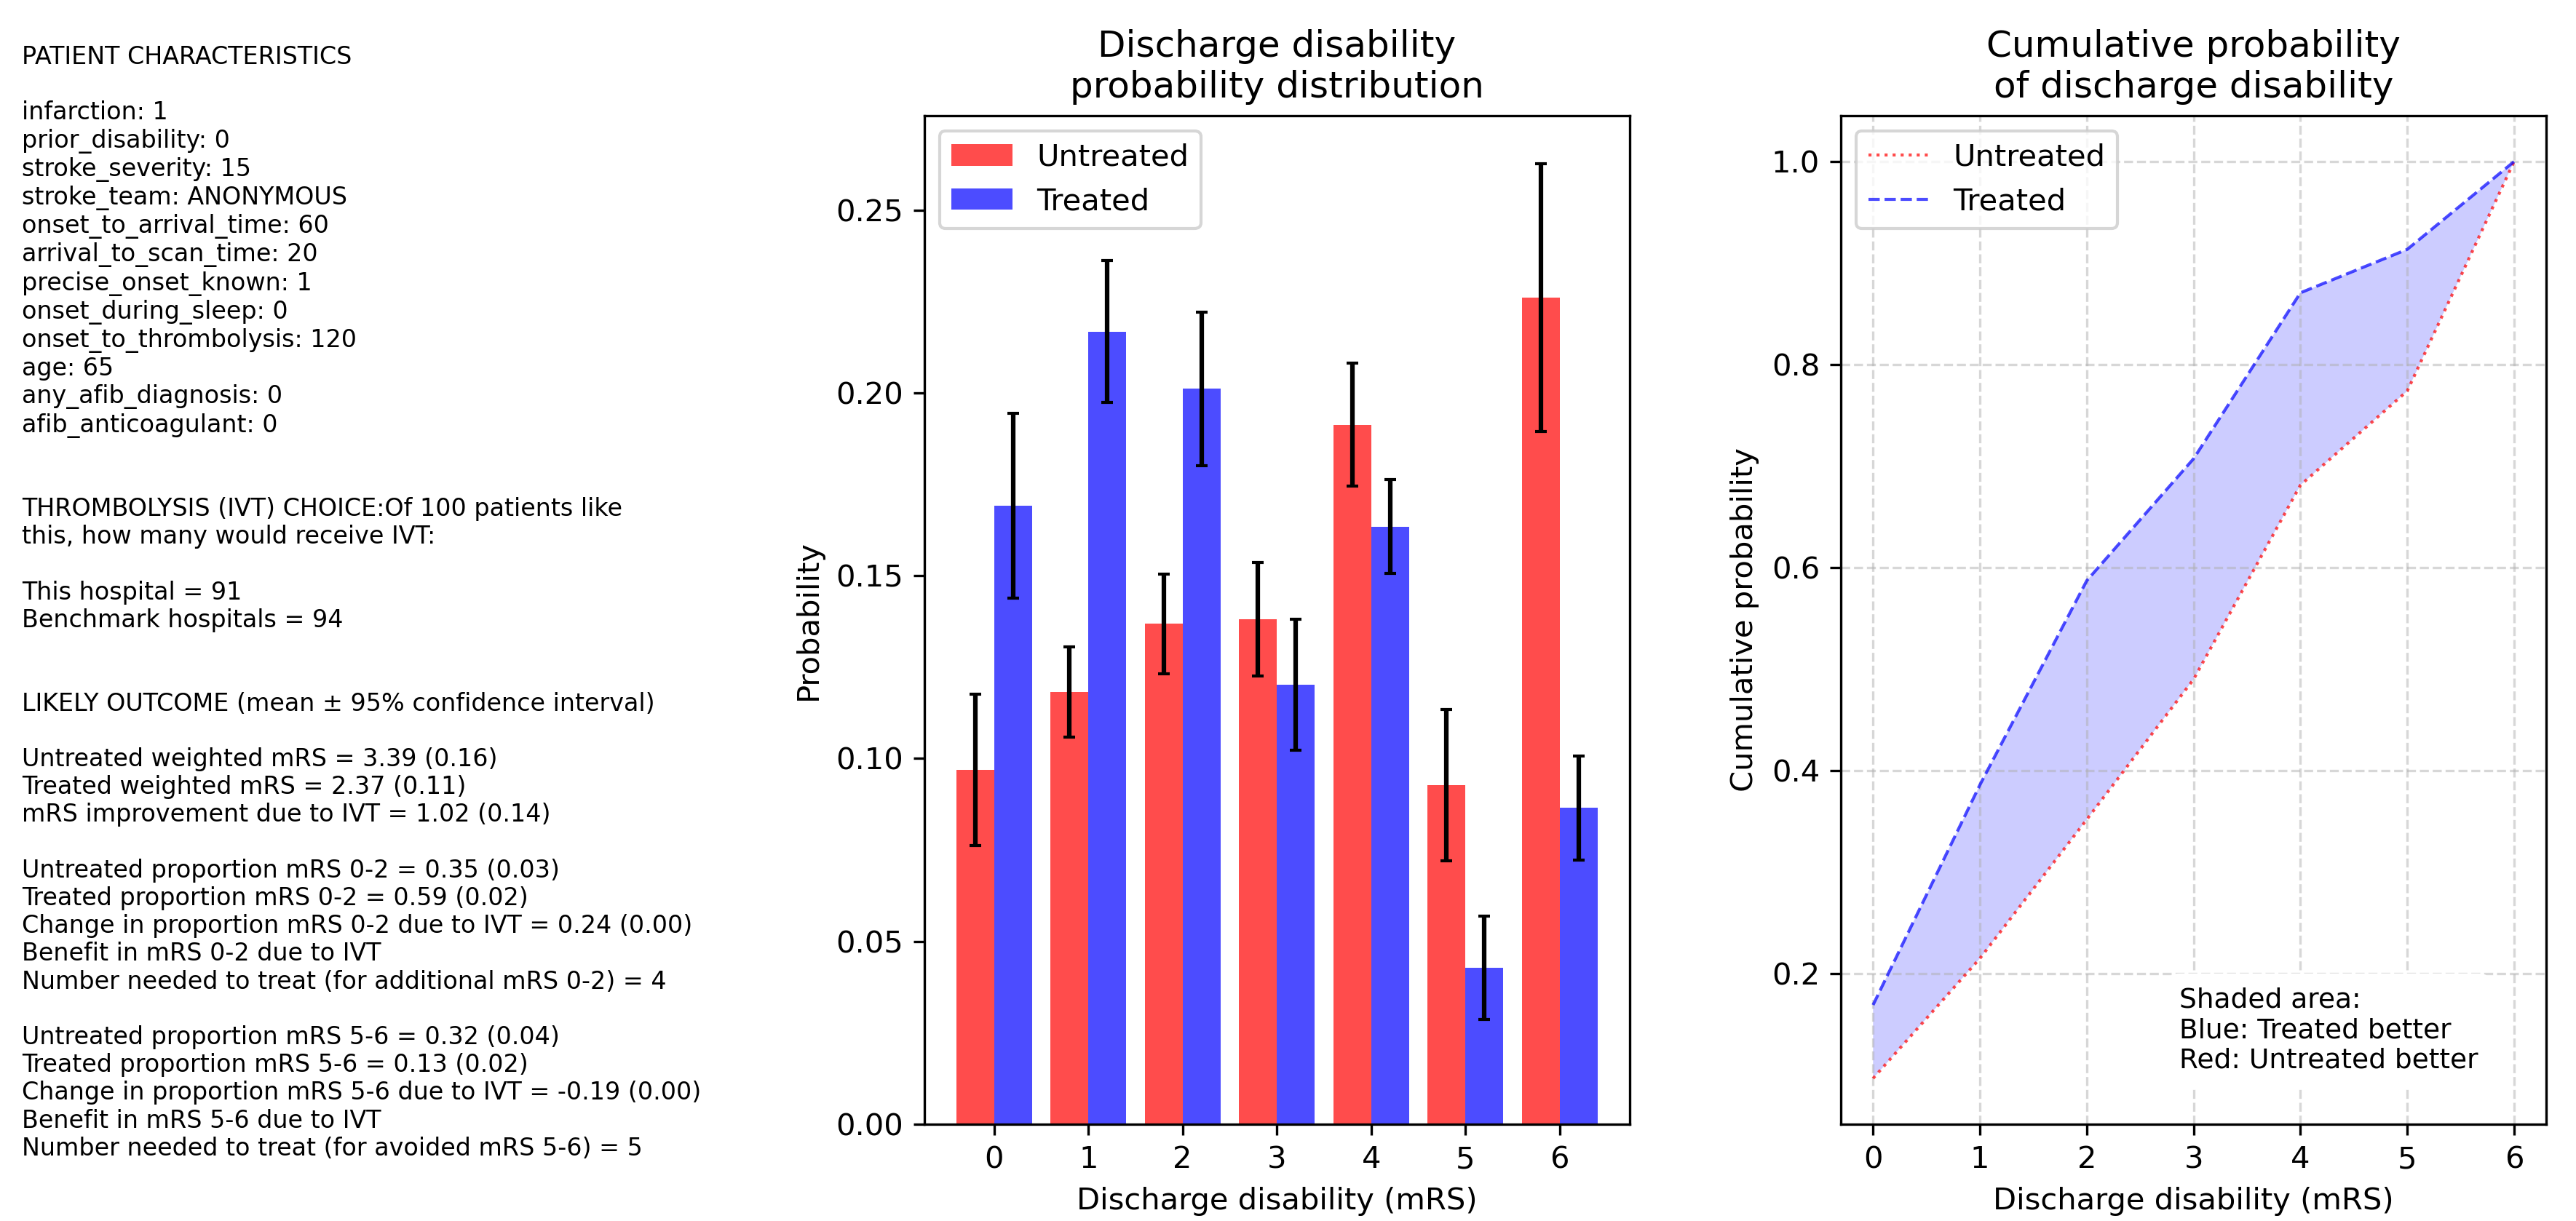
\includegraphics[width=1.0\linewidth]{images/prototype_patient_ideal}
        \caption{\textit{Ideal} candidate for thrombolysis}
        \label{fig:patient_outcome_subfig1}
    \end{subfigure}
    \\
    \vspace{8mm}
    \begin{subfigure}[b]{1.0\textwidth}
        \centering
        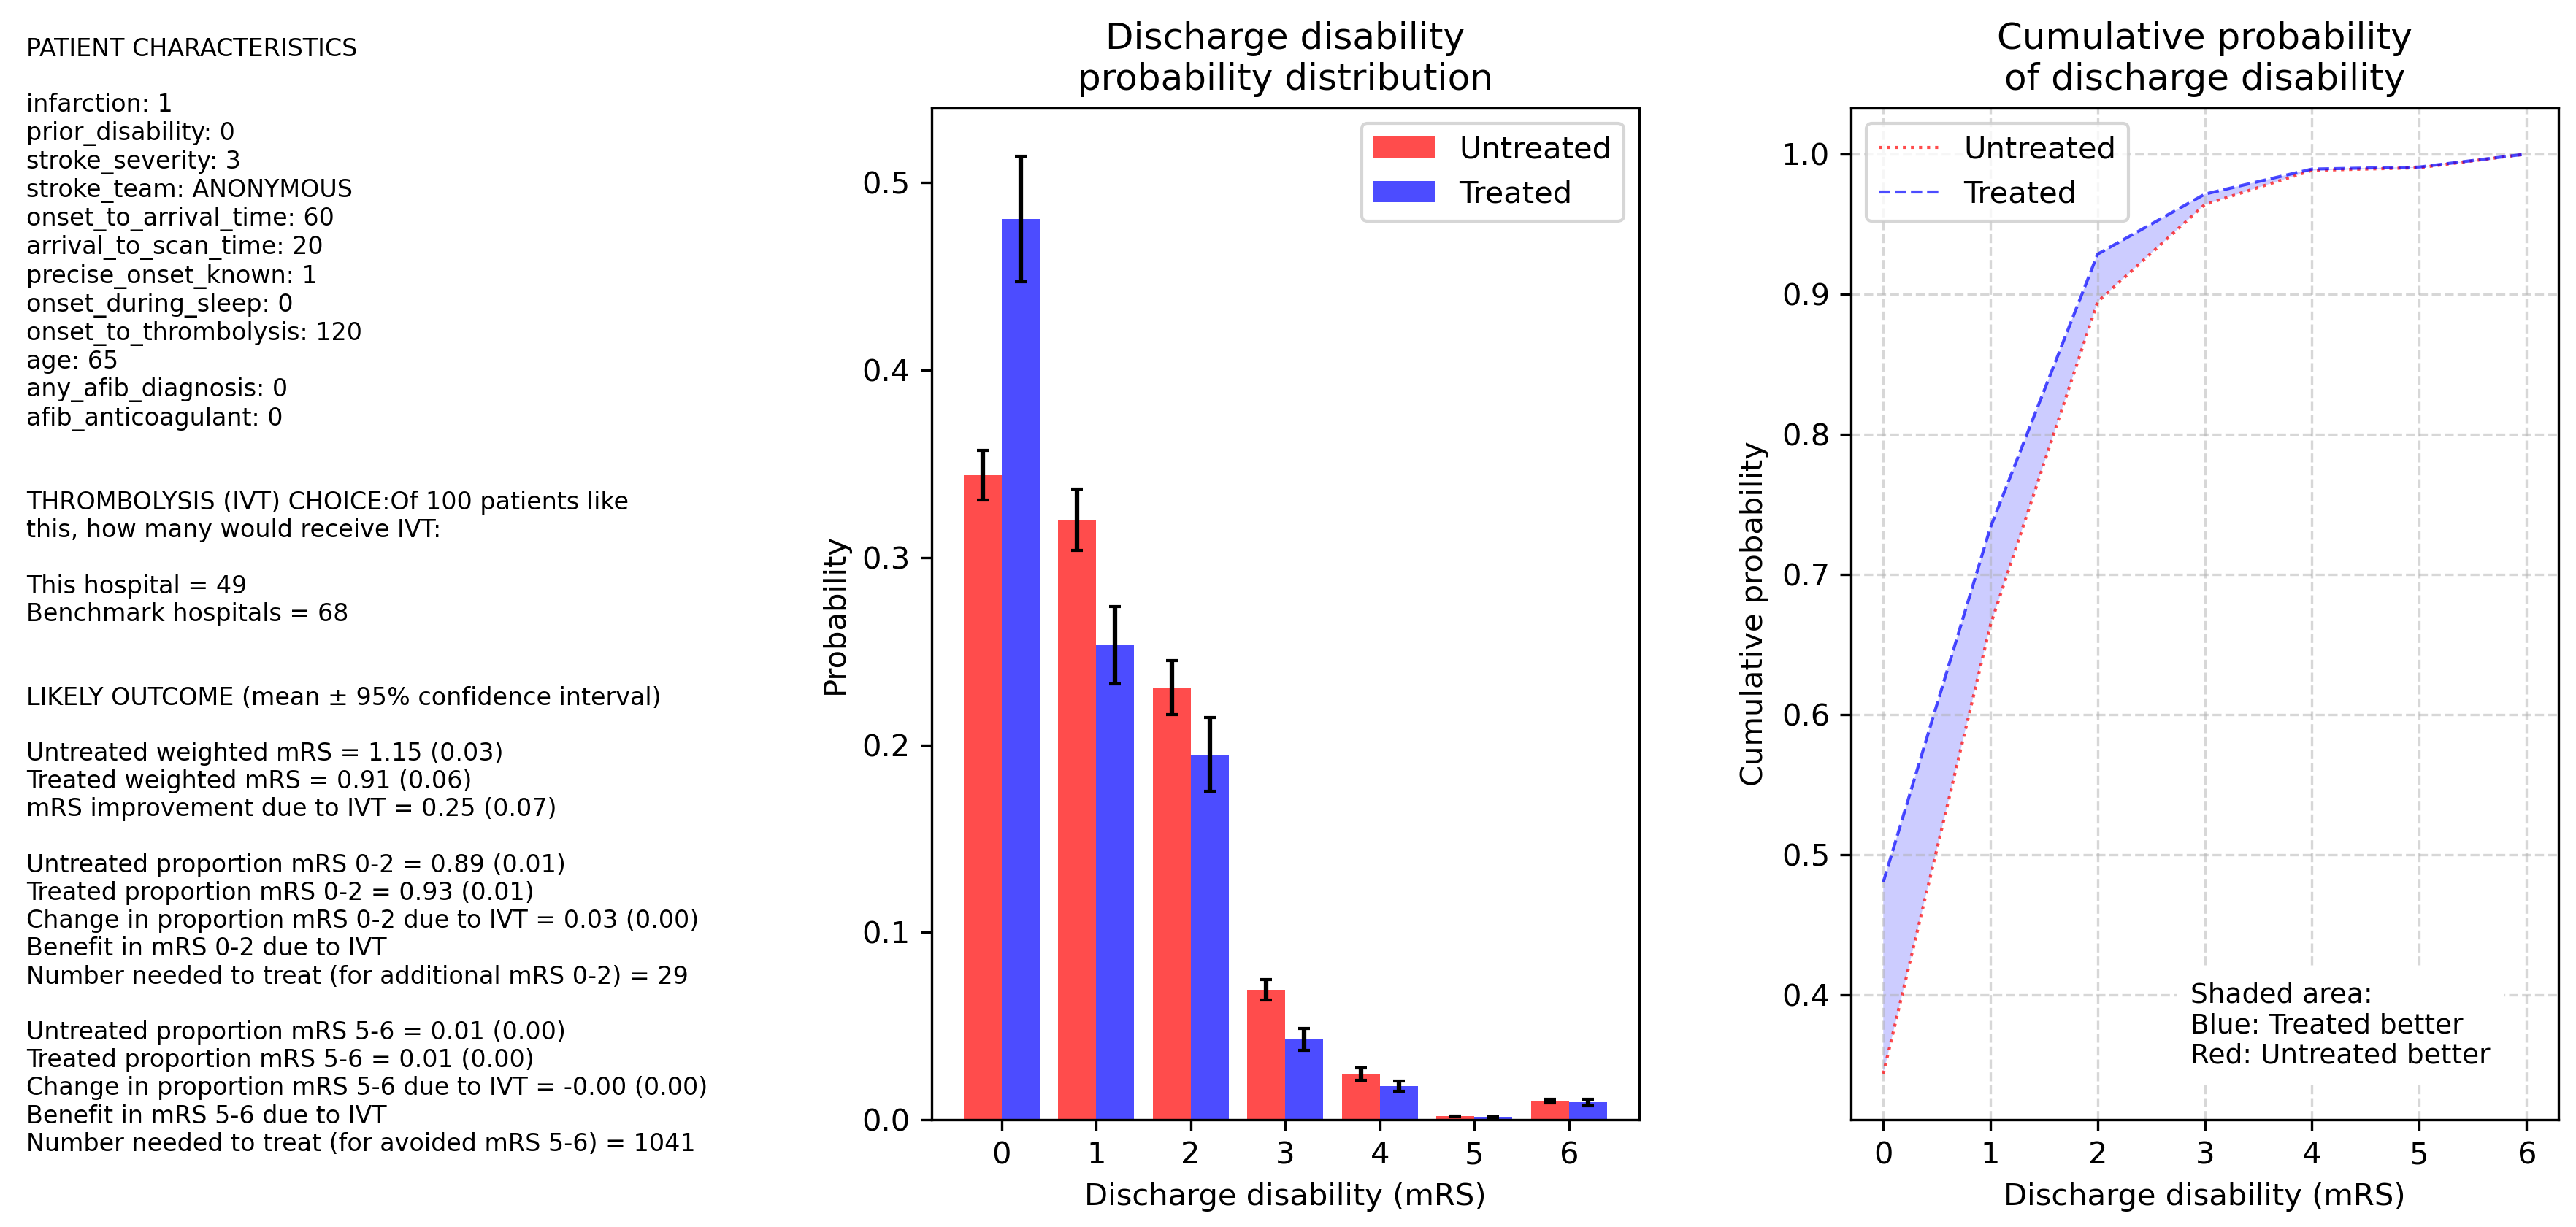
\includegraphics[width=1.0\linewidth]{images/prototype_patient_mild}
        \caption{Patient as \textit{Ideal} candidate for thrombolysis, but with mild stroke (NIHSS 3)}
        \label{fig:patient_outcome_subfig2}
    \end{subfigure}
    \caption{Predicted outcome probabilities, with and without thrombolysis, for an \textit{Ideal} candidate for thrombolysis (top) and for a patient with \textit{mild stroke} (bottom). \textit{Ideal} candidate characteristics: onset-to-arrival = 90 minutes; arrival-to-scan = 15 minutes; onset-to-thrombolysis = 120 minutes; stroke severity (NIHSS) = 15; pre-stroke disability (mRS) = 0; age = 72.5; precisely known onset; onset not during sleep; stroke type = infarction; patient has no atrial fibrillation and is not receiving anticoagulants for atrial fibrillation. Patient with mild stroke is as \textit{Ideal} candidate, but with NIHSS = 3. Errors shown are 95\% confidence limits derived from 30 bootstrapped models.}
    \label{fig:example_patient_outcomes}
\end{figure}



Table \ref{tab:prototype_outcomes} shows predicted outcomes across all prototype patients. All these patients would likely benefit from thrombolysis, but the benefit in mild stroke was smaller.

\begin{minipage}{1\textwidth}
\small
\begin{longtable}{p{5.2cm} | p{1.6cm} p{1.6cm} p{1.5cm} | p{1.6cm} p{1.6cm} p{1.5cm}}
\caption{Predicted outcomes for patient prototypes. \textit{Ideal}: onset-to-arrival = 90 minutes; arrival-to-scan = 15 minutes; onset-to-thrombolysis = 120 minutes; stroke severity (NIHSS) = 15; pre-stroke disability (mRS) = 0; age = 72.5; precisely known onset; onset not during sleep; stroke type = infarction; patient has no atrial fibrillation and is not receiving anticoagulants for atrial fibrillation. \textit{Late arrival}: as \textit{Ideal} but onset-to-arrival = 225 minutes and onset-to-thrombolysis = 255 minutes; \textit{Mild}: As \textit{Ideal} but stroke severity = 3; \textit{Prior disability}: as \textit{Ideal} but pre-stroke disability = 3; \textit{Imprecise}: as \textit{ideal} but stroke onset time estimated. \textit{Age}: as \textit{Ideal} but age = 87.5. Results show probability-weighted disability at discharge, and the proportion of patients predicted to have a very poor outcome (mRS 5-6). With combinations of non-ideal characteristics.}\\
\label{tab:prototype_outcomes}
Patient prototype & Untreated probability-weighted mRS & Treated probability-weighted mRS & Improve-ment & Untreated proportion mRS 5-6 & Treated proportion mRS 5-6 & Improve-ment\\
\endhead
\midrule
Ideal & 3.39 & 2.37 & 1.02 & 0.32 & 0.13 & 0.19\\
Late & 3.39 & 2.73 & 0.66 & 0.32 & 0.18 & 0.14\\
Mild & 1.15 & 0.91 & 0.23 & 0.01 & 0.01 & 0.00\\
Prior disability & 4.22 & 3.61 & 0.61 & 0.41 & 0.23 & 0.19\\
Imprecise & 3.49 & 2.39 & 1.10 & 0.33 & 0.13 & 0.20\\
Age & 4.22 & 3.51 & 0.71 & 0.50 & 0.35 & 0.16\\
Mild + Prior disability & 2.92 & 2.60 & 0.32 & 0.04 & 0.04 & 0.00\\
Mild + Imprecise & 1.28 & 1.01 & 0.26 & 0.02 & 0.01 & 0.00\\
Mild + Age & 1.84 & 1.63 & 0.22 & 0.04 & 0.03 & 0.01\\
Mild + Late & 1.15 & 0.77 & 0.39 & 0.01 & 0.00 & 0.00\\
Imprecise + Prior disability & 4.33 & 3.67 & 0.66 & 0.44 & 0.24 & 0.20\\
Imprecise + Age & 4.31 & 3.57 & 0.74 & 0.53 & 0.36 & 0.17\\
Imprecise + Late & 3.49 & 2.75 & 0.74 & 0.33 & 0.17 & 0.17\\
Prior disability + Age & 4.62 & 4.35 & 0.27 & 0.53 & 0.44 & 0.08\\
Prior disability + Late & 4.22 & 3.70 & 0.52 & 0.41 & 0.27 & 0.14\\
Mild + Prior disability + Imprecise & 3.01 & 2.65 & 0.36 & 0.06 & 0.06 & 0.00\\


\end{longtable}
\normalsize
\end{minipage}

\subsection{Mild stroke}

Table \ref{tab:mild_stroke} shows the predicted benefit of thrombolysis, for those who actually received thrombolysis, in mild ischaemic stroke (NIHSS 0-4) and non-mild stroke (NIHSS 5+) at \textit{benchmark hospitals} and \textit{non-benchmark hospitals}. In those mild stroke patients who actually received thrombolysis, either at a benchmark hospital or a non-benchmark hospital, it was predicted that there would be an increased proportion of good outcomes, and a beneficial shift in average mRS, but that there would be a small increase in bad outcomes. For non-mild stroke, thrombolysis improved by all outcome measures.

\begin{minipage}{1\textwidth}
\small
\renewcommand{\arraystretch}{1.2}
\begin{longtable}{p{7.2cm} | p{1.6cm} p{1.6cm} | p{1.6cm} p{1.6cm}}
\caption{Patient characteristics and predicted outcomes for mild stroke (NIHSS 0-4) and non-mild stroke (NIHSS 5+). Results shown are the mean for all patients who actually received treatment at either a non-benchmark hospital or a benchmark hospital.}\\
\label{tab:mild_stroke}

Metric & Non-benchmark NIHSS 0-4 & Non-benchmark NIHSS 5+ & Benchmark NIHSS 0-4 & Benchmark NIHSS 5+\\
\endhead
\midrule
Stroke severity & 3.1 & 12.8 & 2.9 & 12.5\\
Onset to thrombolysis (minutes) & 147 & 138 & 140 & 130\\
Proportion onset known precisely & 86\% & 84\% & 77\% & 71\%\\
Proportion untreated mRS 0-1 & 0.556 & 0.240 & 0.564 & 0.234\\
Proportion untreated mRS 0-2 & 0.797 & 0.401 & 0.795 & 0.399\\
Proportion untreated mRS 5-6 & 0.026 & 0.281 & 0.024 & 0.284\\
Untreated weighted mRS & 1.535 & 3.188 & 1.537 & 3.205\\
Change in proportion mRS 0-1 (+ve is better) & 0.019 & 0.063 & 0.027 & 0.072\\
Change in proportion mRS 0-2 (+ve is better) & 0.012 & 0.079 & 0.009 & 0.078\\
Change in proportion mRS 5-6 (-ve is better) & 0.010 & -0.056 & 0.009 & -0.057\\
Change in weighted mRS ( -ve is better) & -0.036 & -0.341 & -0.053 & -0.354\\

\end{longtable}
\normalsize
\end{minipage}


\subsection{Lifetime economic model}

Table \ref{tab:health_econ} shows the modelled health economics of thrombolysis use, comparing actual use of thrombolysis with \textit{benchmark} thrombolysis use. The effect of thrombolysis was estimated by predicting the outcomes with and without thrombolysis for the two groups (those that actually received thrombolysis, and those predicted to receive thrombolysis using \textit{benchmark} decisions). Benchmark decisions maintain the benefit of using thrombolysis, but extend that benefit to more patients. This extended benefit was not at the cost of any predicted increase in the worst outcomes (mRS 5-6). The extended benefit led to more QALYs added across the population by treatment, and more predicted savings to NHS healthcare costs.

\begin{table}[!h]
\small
\caption{Health economic analysis: Analysis for  populations based on predicted benefit (or dis-benefit) of thrombolysis. The effect of thrombolysis was estimated by predicting the outcomes with and without thrombolysis for the two groups (those that actually received thrombolysis, and those predicted to receive thrombolysis using \textit{benchmark} decisions). The analysis compares the populations currently treated, or the population that would be treated using \textit{benchmark} decisions (the majority vote of the predicted choice of the the 25 stroke teams most likely to use thrombolysis). Results are shown for (a) the treated populations, and (b) adjusted for 1,000 emergency stroke admissions }
\label{tab:main}

\begin{subtable}{1\textwidth}
\centering
\caption{Counterfactual analysis of the effect of thrombolysis in either those patients who actually received thrombolysis, or those patients where the \textit{benchmark decision} would be to use thrombolysis.}
\begin{tabular}{p{2.0cm} p{1.5cm} p{1.2cm} p{1.3cm} p{1.5cm} p{1.3cm} p{1.4cm} p{1.3cm} p{1.3cm}}
\toprule
Population & \raggedright Modelled treatment & Death & Survival (median years) & Care years (median) & QALYs & \raggedright Discounted cost per patient & Proportion mRS 0-2 & Proportion mRS 5-6\tabularnewline
\midrule
Actual use & Untreated & 17.1\% & 7.60 & 0.28 & 5.020 & £20,370 & 47.1\% & 23.9\%\tabularnewline
& Treated & 14.2\% & 7.91 & 0.25 & 5.258 & £19,806 & 53.9\% & 19.3\%\tabularnewline
& Difference & -2.9\% & 0.31 & -0.03 & 0.238 & -£565 & 6.8\% & -4.7\%\tabularnewline
\midrule
Benchmark & Untreated & 17.4\% & 7.63 & 0.28 & 5.036 & £20,388 & 46.5\% & 24.1\%\tabularnewline
& Treated & 14.4\% & 7.93 & 0.25 & 5.269 & £19,784 & 53.4\% & 19.4\%\tabularnewline
& Difference & -3.0\% & 0.30 & -0.03 & 0.234 & -£603 & 6.9\% & -4.8\%\tabularnewline

\end{tabular}
\end{subtable}

\vspace{3mm}

\begin{subtable}{1\textwidth}
\centering
\caption{Analysis for 1,000 emergency stroke admissions (all stroke types)}
\begin{tabular}{p{1.9cm} p{1.9cm} p{1.9cm} p{1.9cm} p{1.9cm} p{1.9cm} p{2.2cm}}
\toprule
Population & Proportion treated & QALYs added & Healthcare costs saved & \raggedright Thrombolysis cost (£450 per patient) & \raggedright Cost per QALY added & \raggedright Net cost of thrombolysis\tabularnewline
\midrule
Actual & 11.0\% & 26.3 & £62,294 & £49,658 & £1,890 & -£12,637\tabularnewline
Benchmark & 13.6\% & 31.7 & £81,914 & £61,117 & £1,927 & -£20,797\tabularnewline
\bottomrule
\end{tabular}
\end{subtable}
\label{tab:health_econ}
\end{table}

\normalsize

\subsection{Pathway model}

Figure \ref{fig:thrombolysis_rates_teams} compares observed and predicted thrombolysis use (based on historic performance, and applying \textit{benchmark decisions}). Predicted and observed thrombolysis use correlate very closely (r-squared 0.94). Predicted rates were, on average, slightly higher (1.7\%) than observed rates.

\begin{figure}[!h]
    \centering
    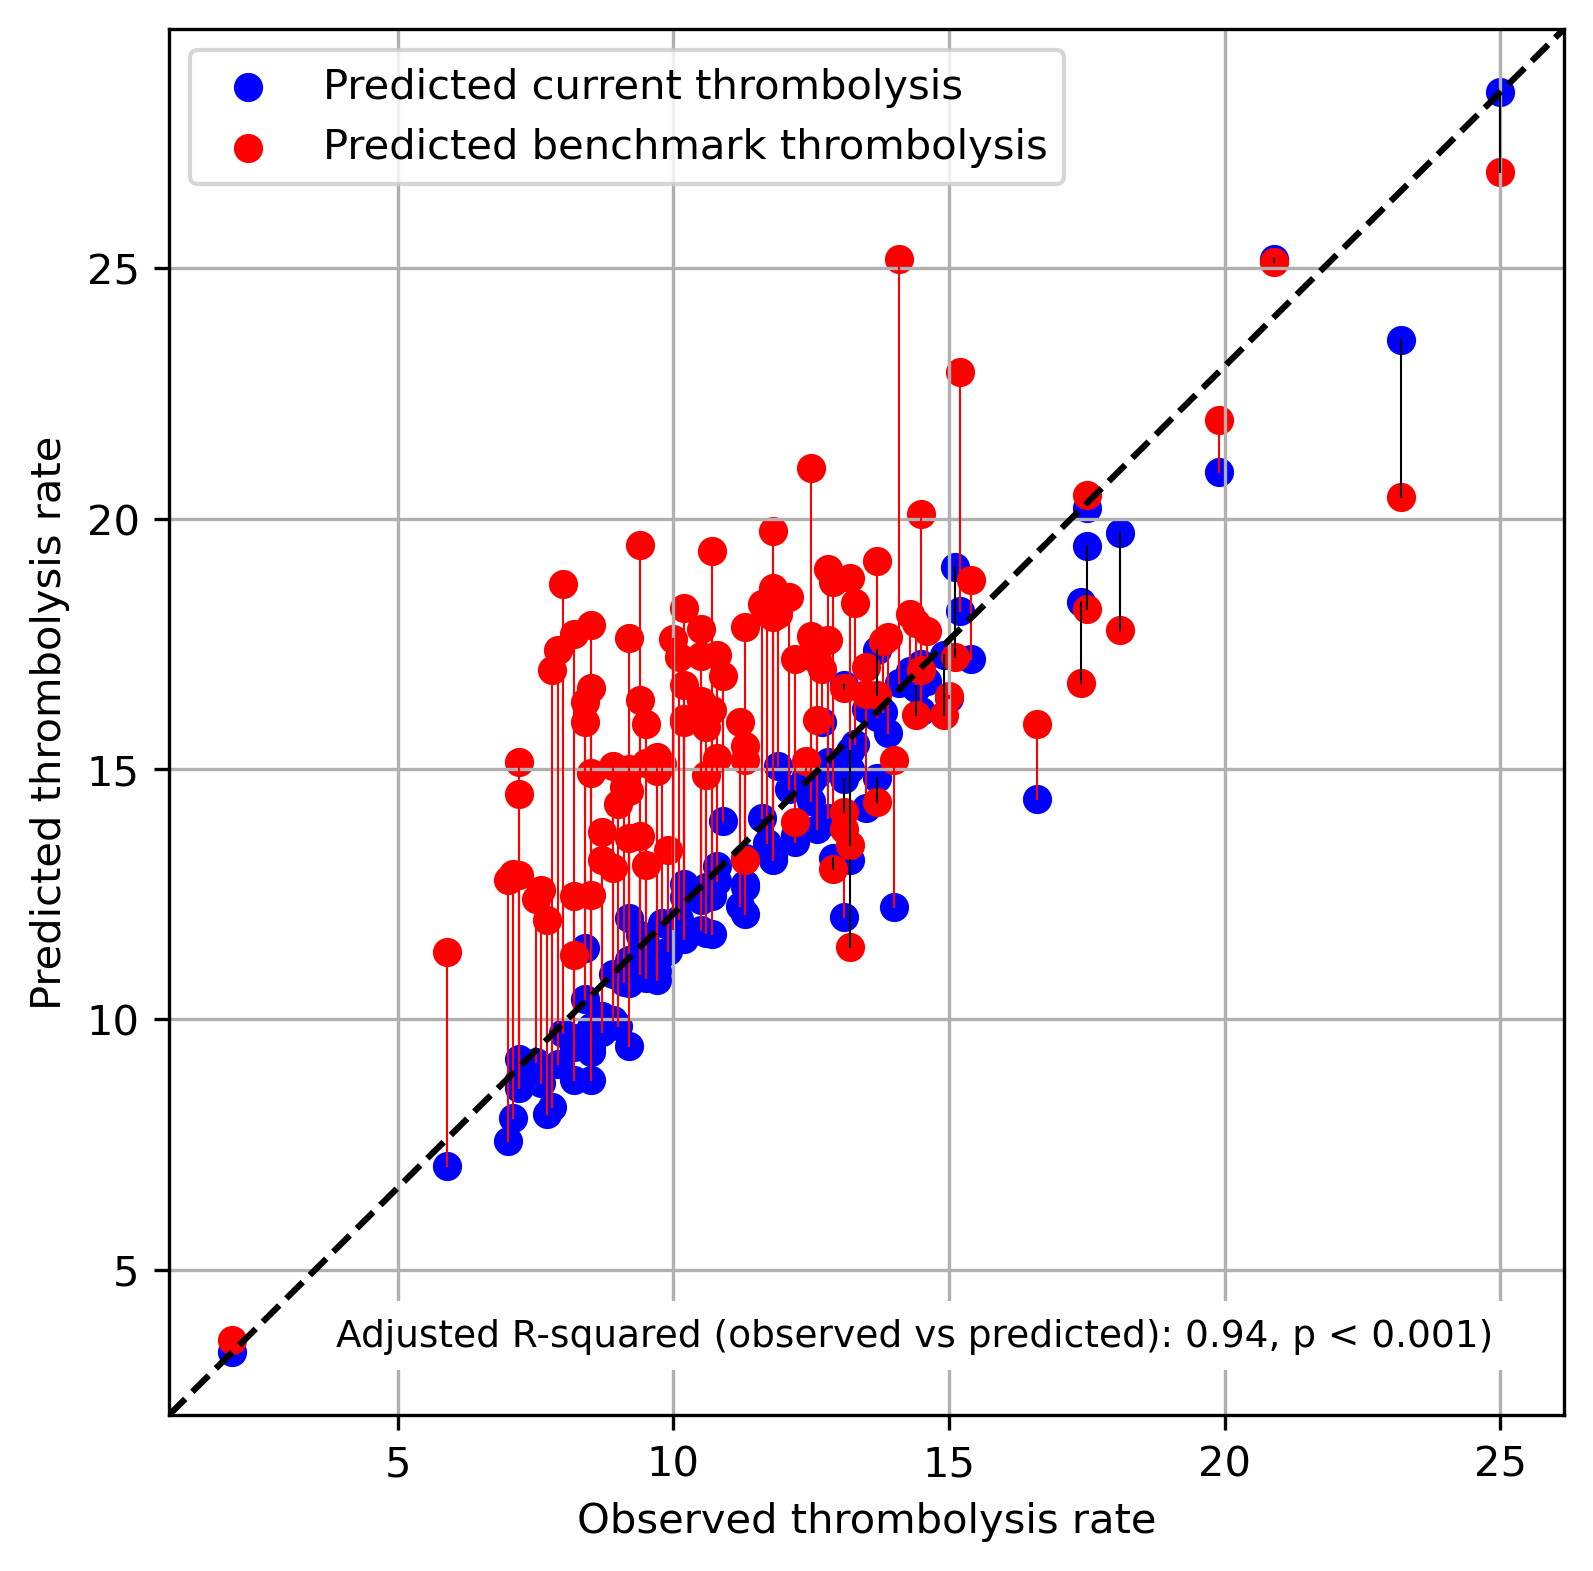
\includegraphics[width=0.5\linewidth]{images/thrombolysis_rates_model}
    \caption{Comparison of observed and predicted thrombolysis use across stroke teams. Blue circles show predictions based on historic hospital performance. Red circles show the expected thrombolysis use if \textit{benchmark decisions} were made. The black dotted line shows least-squares regression analysis between observed and predicted (using historic performance) thrombolysis use.}
    \label{fig:thrombolysis_rates_teams}
\end{figure}


Across the study population, by combining pathway improvements, thrombolysis use in all those emergency stroke admissions arriving by ambulance shows the potential to be increased from 13\% to 20\% (figure \ref{fig:scenarios_population}). Using a model based on clinical trial data, benefit, as measured by number of number of people discharged with no, or minimal, disability (mRS 0 or 1)  could be doubled from 10 to 20 additional excellent outcomes per 1,000 admissions. The single most influential change was applying \textit{benchmark} decisions. Improving speed would not significantly increase the number of people given thrombolysis, but would lead to more benefit from thrombolysis (as all treated patients will have improved benefit). Figure \ref{fig:scenarios_team} shows this analysis applied to a single stroke team.


\begin{figure}[!h]
    \centering
    \begin{subfigure}[b]{1\textwidth}
        \centering
        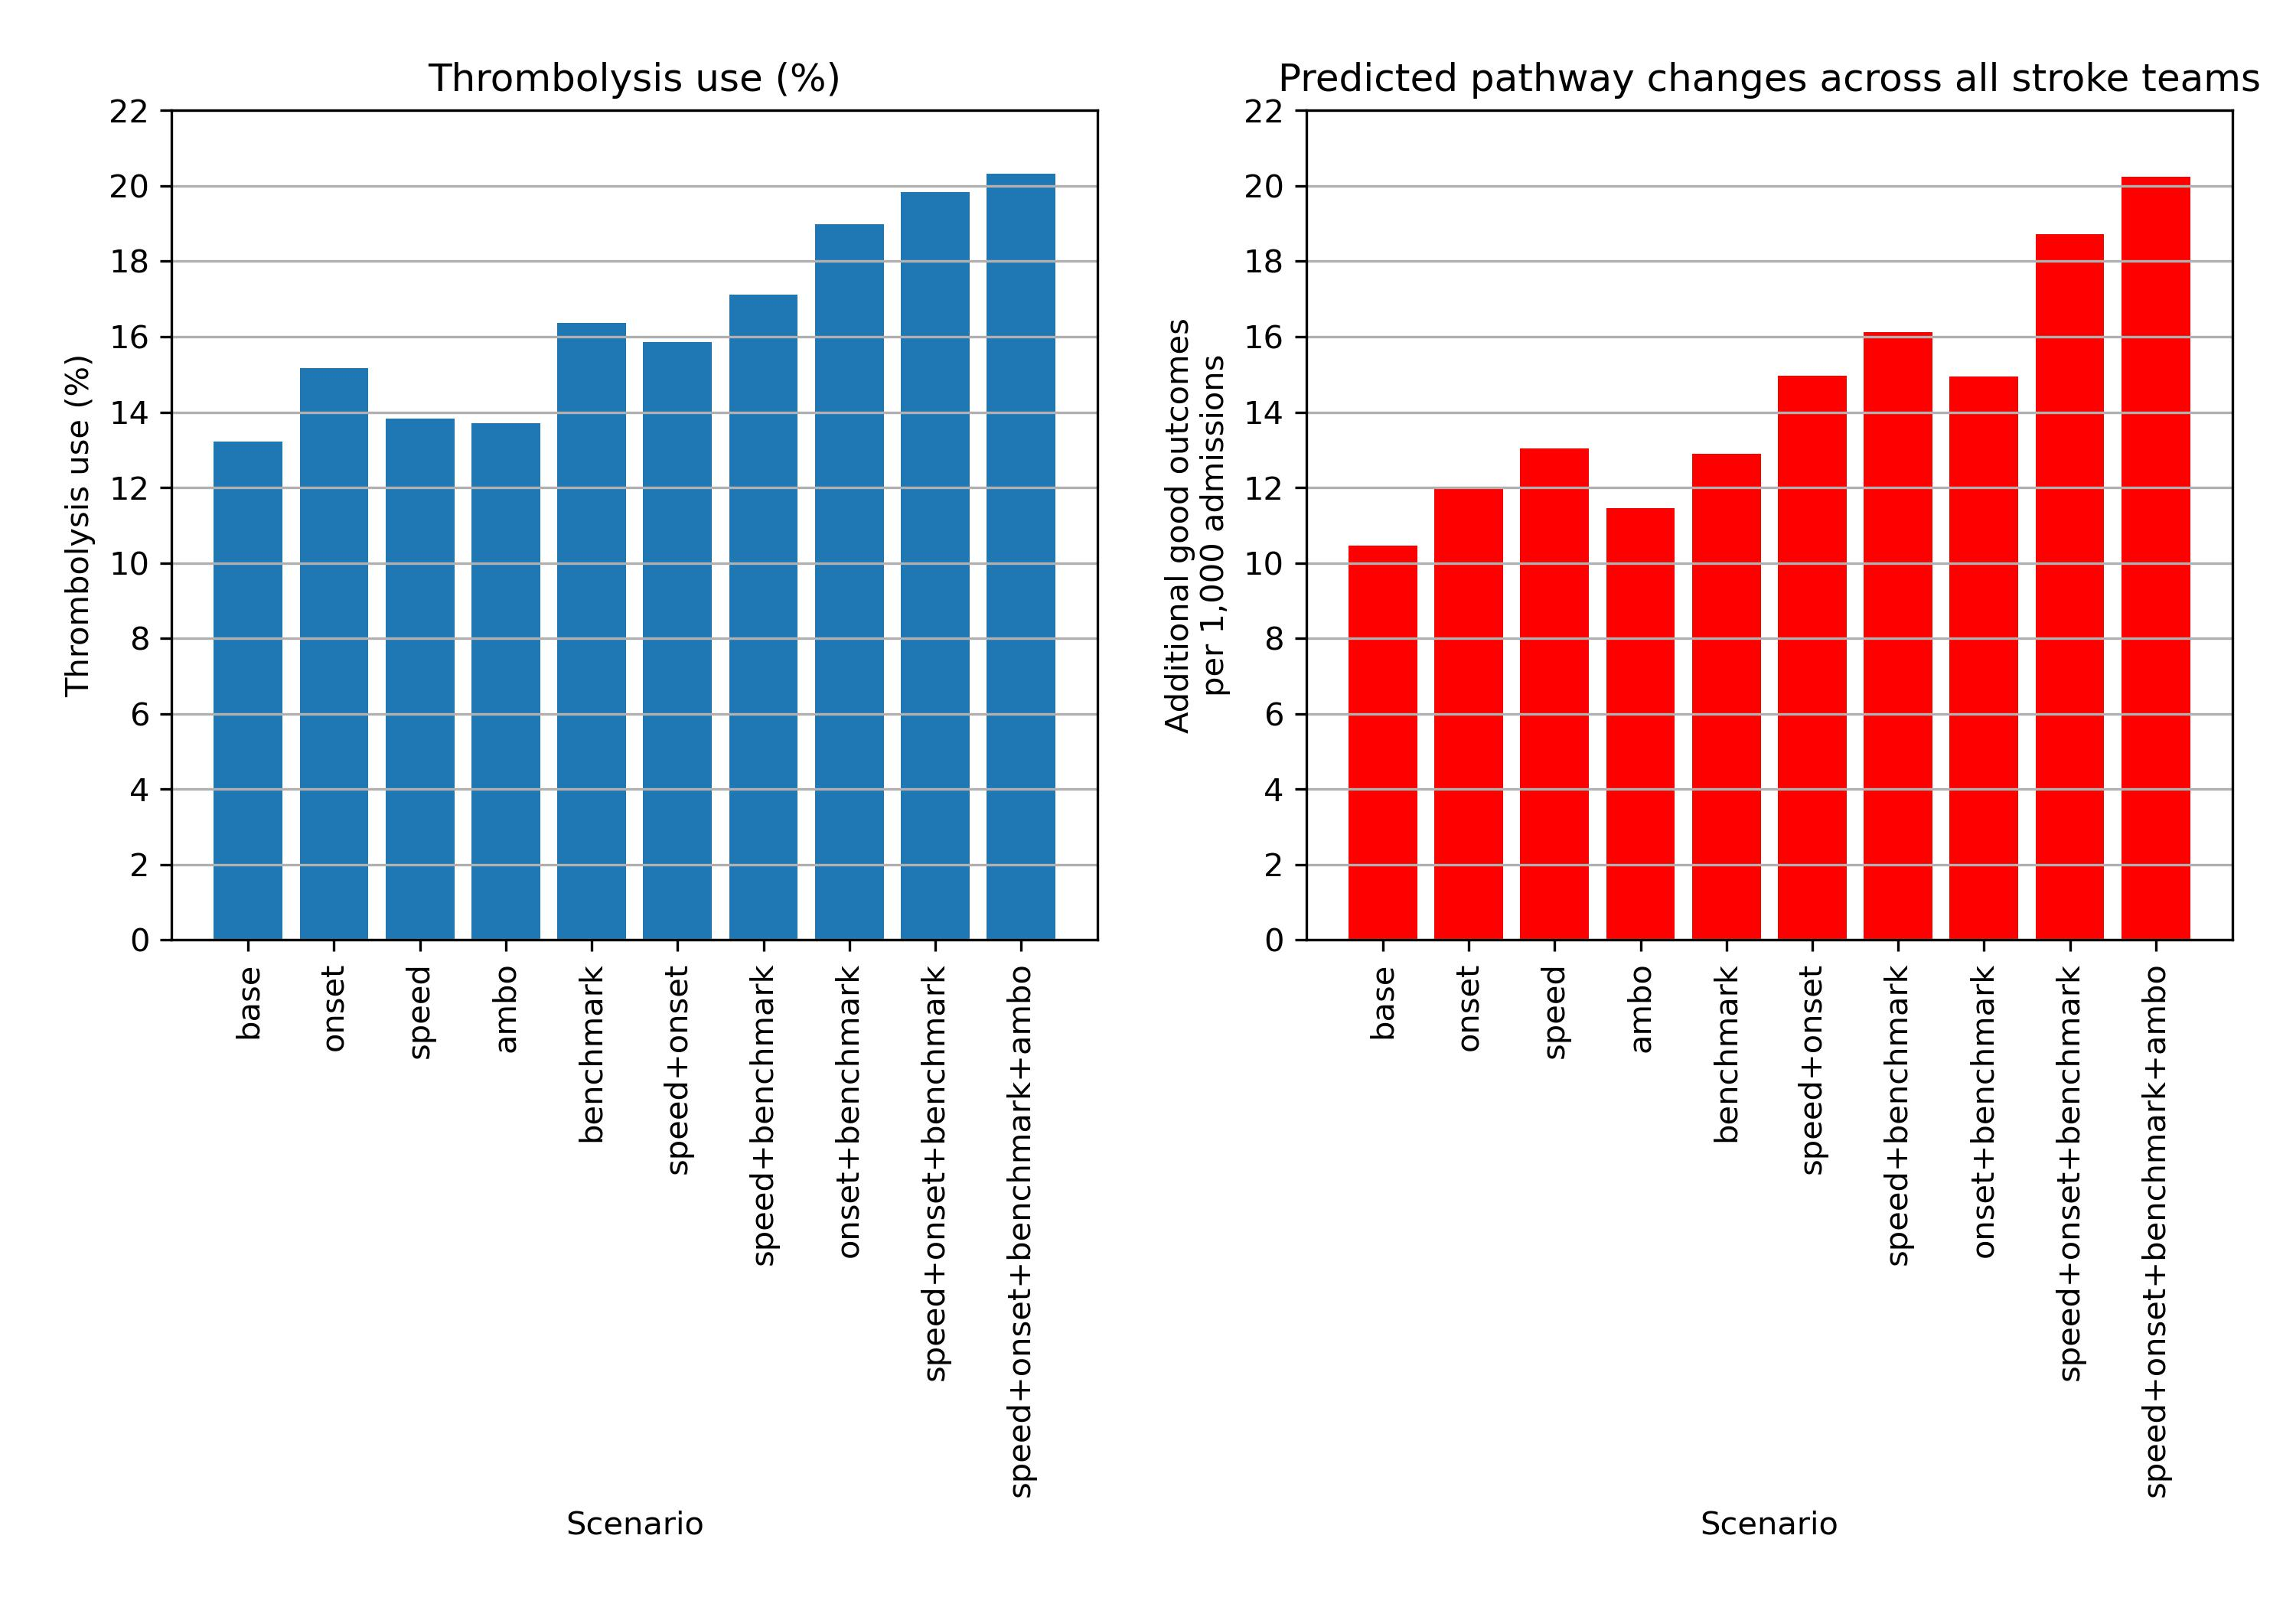
\includegraphics[width=0.8\linewidth]{images/sim_results_summary}
        \caption{Changes across the study population}
        \label{fig:scenarios_population}
    \end{subfigure}
    \\
    \vspace{8mm}
    \begin{subfigure}[b]{1\textwidth}
        \centering
    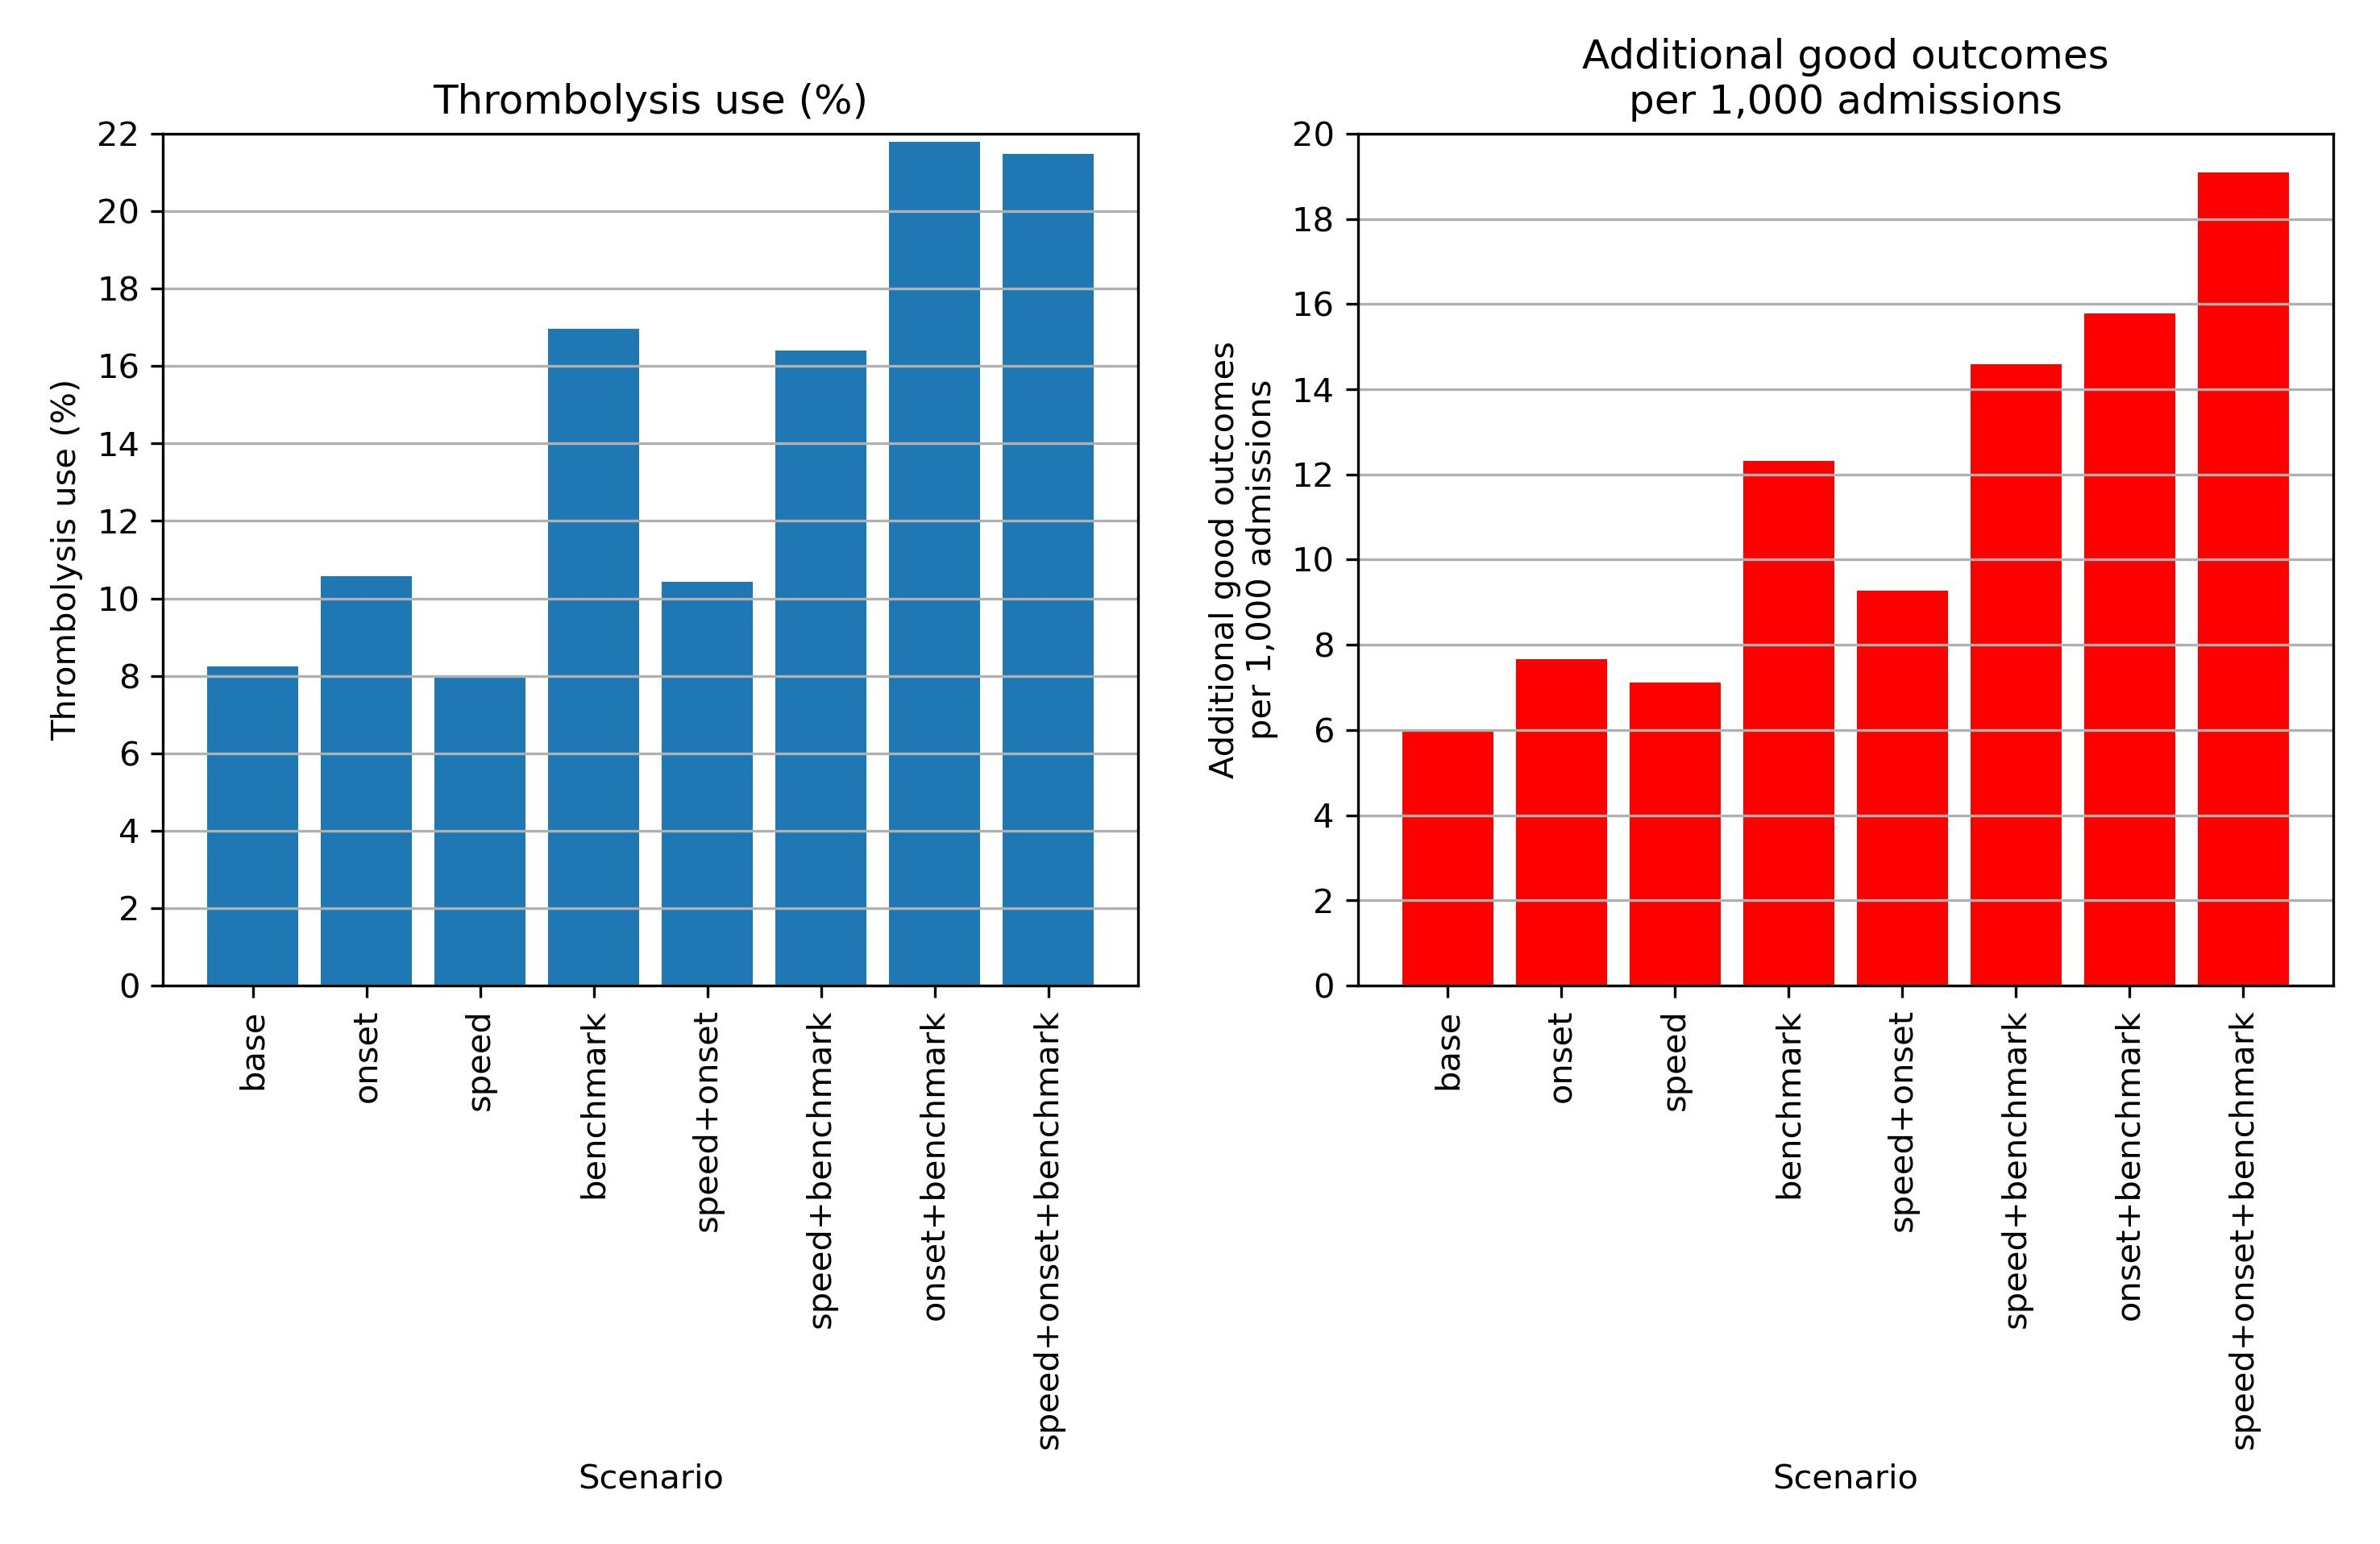
\includegraphics[width=0.8\linewidth]{images/sim_results_team_x}
        \caption{Changes in one stroke team}
        \label{fig:scenarios_team}
    \end{subfigure}
    \caption{Expected effect of alternative process improvement initiatives across the study population (top) or one specific stroke team (bottom). Each chart shows the effect on thrombolysis use (left) and on number of additional good outcomes (mRS 0-1) per 1,000 admissions due to use of thrombolysis (right). \textit{Base}: Uses the hospitals’ recorded pathway statistics. \textit{Onset}: Sets the proportion of patients with a known stroke onset time to the national upper quartile if currently less than the national upper quartile. \textit{Speed}: Sets 95\% of patients having a scan within 4 hours of arrival, and all patients have 15 minutes arrival-to-scan time and 15 minutes scan-to-needle time. \textit{Ambo}: Subtracts 15 minutes from the current ambulance call to arrival-at-hospital times. \textit{Benchmark}: The benchmark thrombolysis rate takes the likelihood to give thrombolysis for patients scanned within 4 hours of onset from the majority vote of the 25 benchmark hospitals.}
    \label{fig:sim_results_summary}
\end{figure}



\section{Discussion}



\section{References}
\bibliographystyle{naturemag}
%\bibliographystyle{plainnat}
%\bibliographystyle{unsrt}
%\bibliographystyle{unsrtnat}
\bibliography{references}


% Word counts - Don't count these!
%TC:ignore
\section{Word counts}
\detailtexcount{main}
%TC:endignore


\end{document}